\documentclass[12pt]{article}
\usepackage{graphicx,chemarrow}
\usepackage{ifthen}
\pagestyle{empty}

\usepackage[]{mcode}

\topmargin -0.6in
\headsep 0.40in
\oddsidemargin 0.0in
\textheight 9.0in
\textwidth 6.5in
\newcommand{\mybox}[1]{\fbox{\parbox[h]{0.9\textwidth}{#1}}}
\newcommand{\beqn}{\begin{eqnarray}}
\newcommand{\eeqn}{\end{eqnarray}}
\newcommand{\vf}{\varphi}
\def \beq {\begin{eqnarray}}
\def \eeq {\end{eqnarray}}
\def \beqn {\begin{eqnarray*}}
\def \eeqn {\end{eqnarray*}}
\newcommand{\comment}[1]{}
\newcommand{\solution}[1]{#1}
\begin{document}

\centerline{\Large \bf Systems Biology, Homework \# 4}
\vskip 4 pt
\centerline{\Large \bf Mathematical Analysis}
\vskip 4 pt
\centerline{\Large  Due Sunday March 6th 11:59 pm}

\begin{enumerate}

\item Phase analysis can be applied to systems of a single dimension.  The phase portrait of a one-dimensional system lies on a  {\em phase line}.   For example, the phase portrait of the system 
\beqn
\frac{dx(t)}{dt} = x^2(t) - x(t) = x(t) (x(t)-1),
\eeqn
is shown below, with the open circle indicating an unstable steady state, the closed circle indicating a stable steady state, and the arrows indicating the direction of motion.

\begin{center}
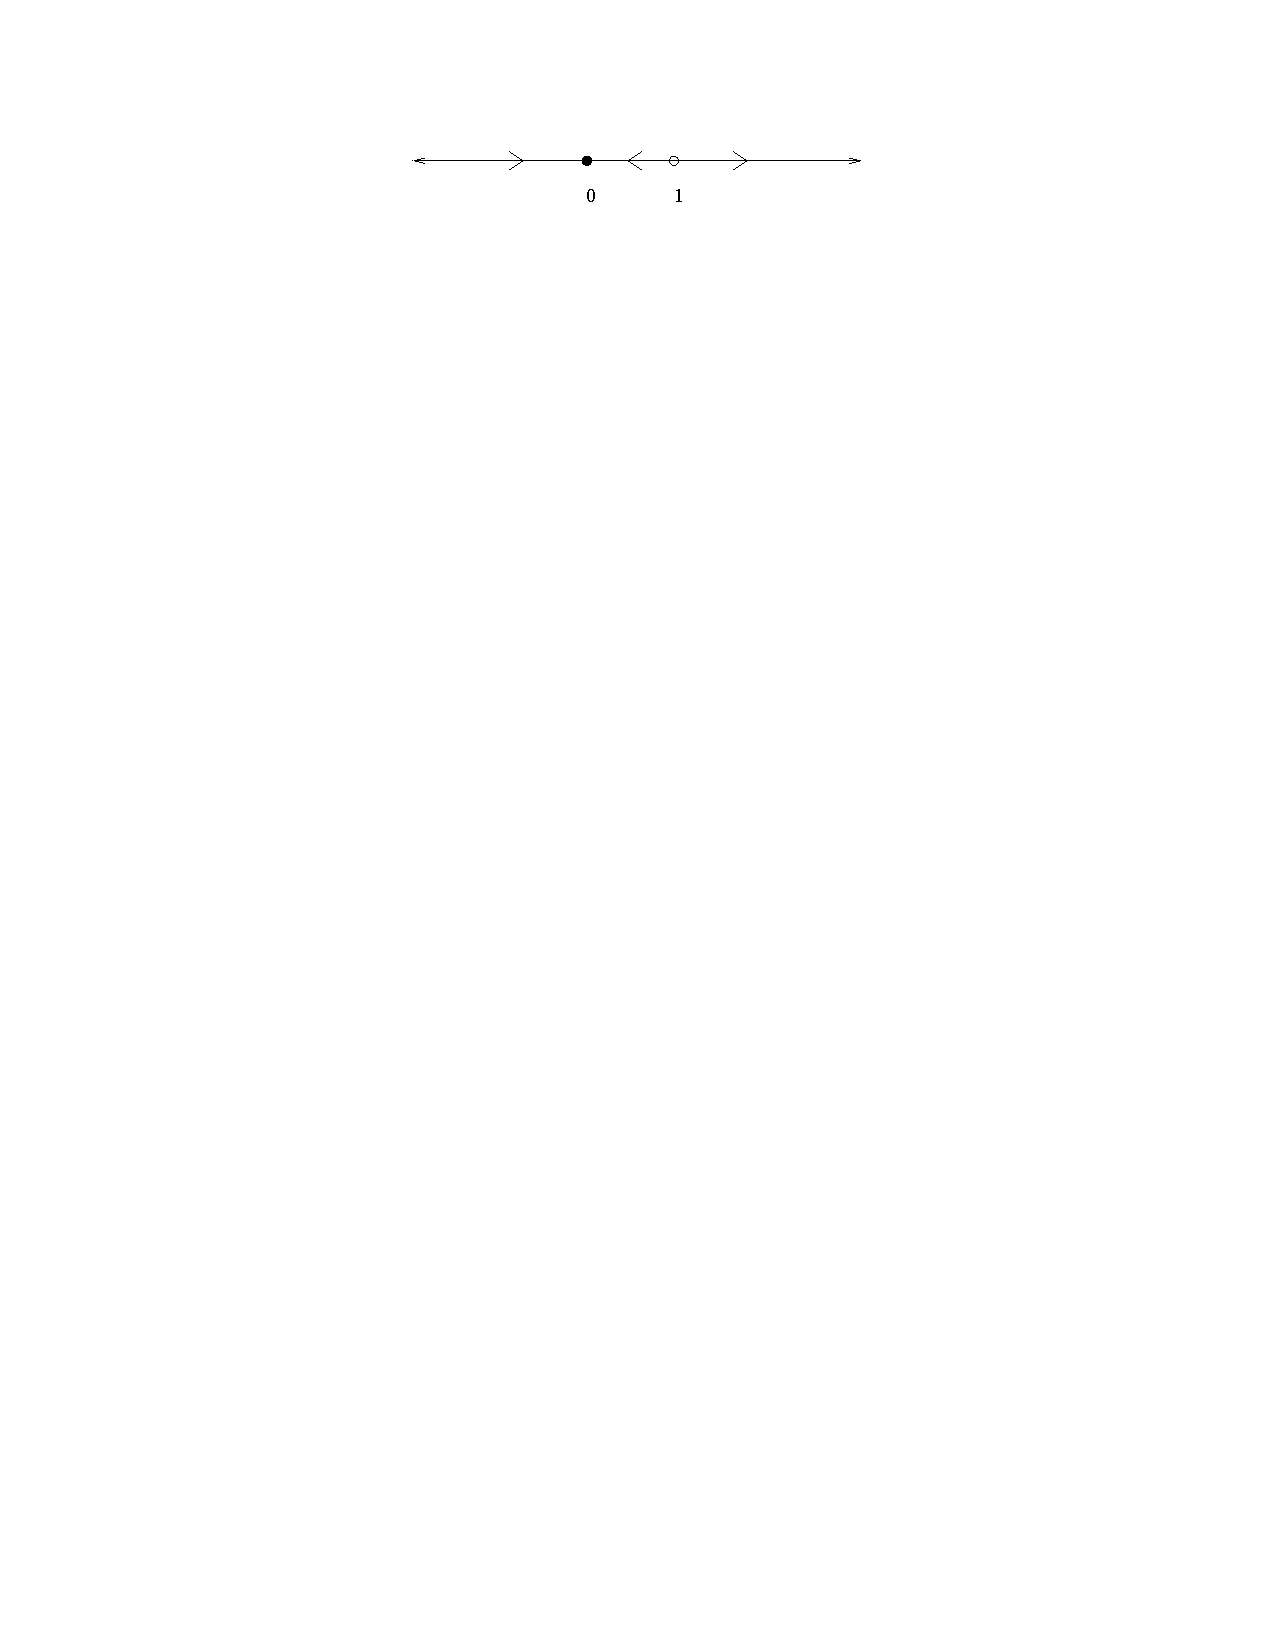
\includegraphics[width=3in]{1dphase}
\end{center}

\begin{enumerate}
\item Sketch the phase line for the differential equation
\beqn
  \frac{d}{dt} V(t) &=& V^3(t) - V(t) 
\eeqn


\item Consider the simple model
\beqn
%\label{eq:plsys}
\frac{d}{dt} s(t) = k - \frac{V_{\mbox{\tiny max}} s}{K_M + s}
\eeqn
in which species $s$ is produced at a fixed rate and consumed via Michaelis-Menten kinetics.  Sketch a phase line for this system. Verify that the steady state is stable for any non-negative parameter values, provided  $V_{\mbox{\tiny max}} > k$.
\end{enumerate}

\item Consider the network:
\begin{center}
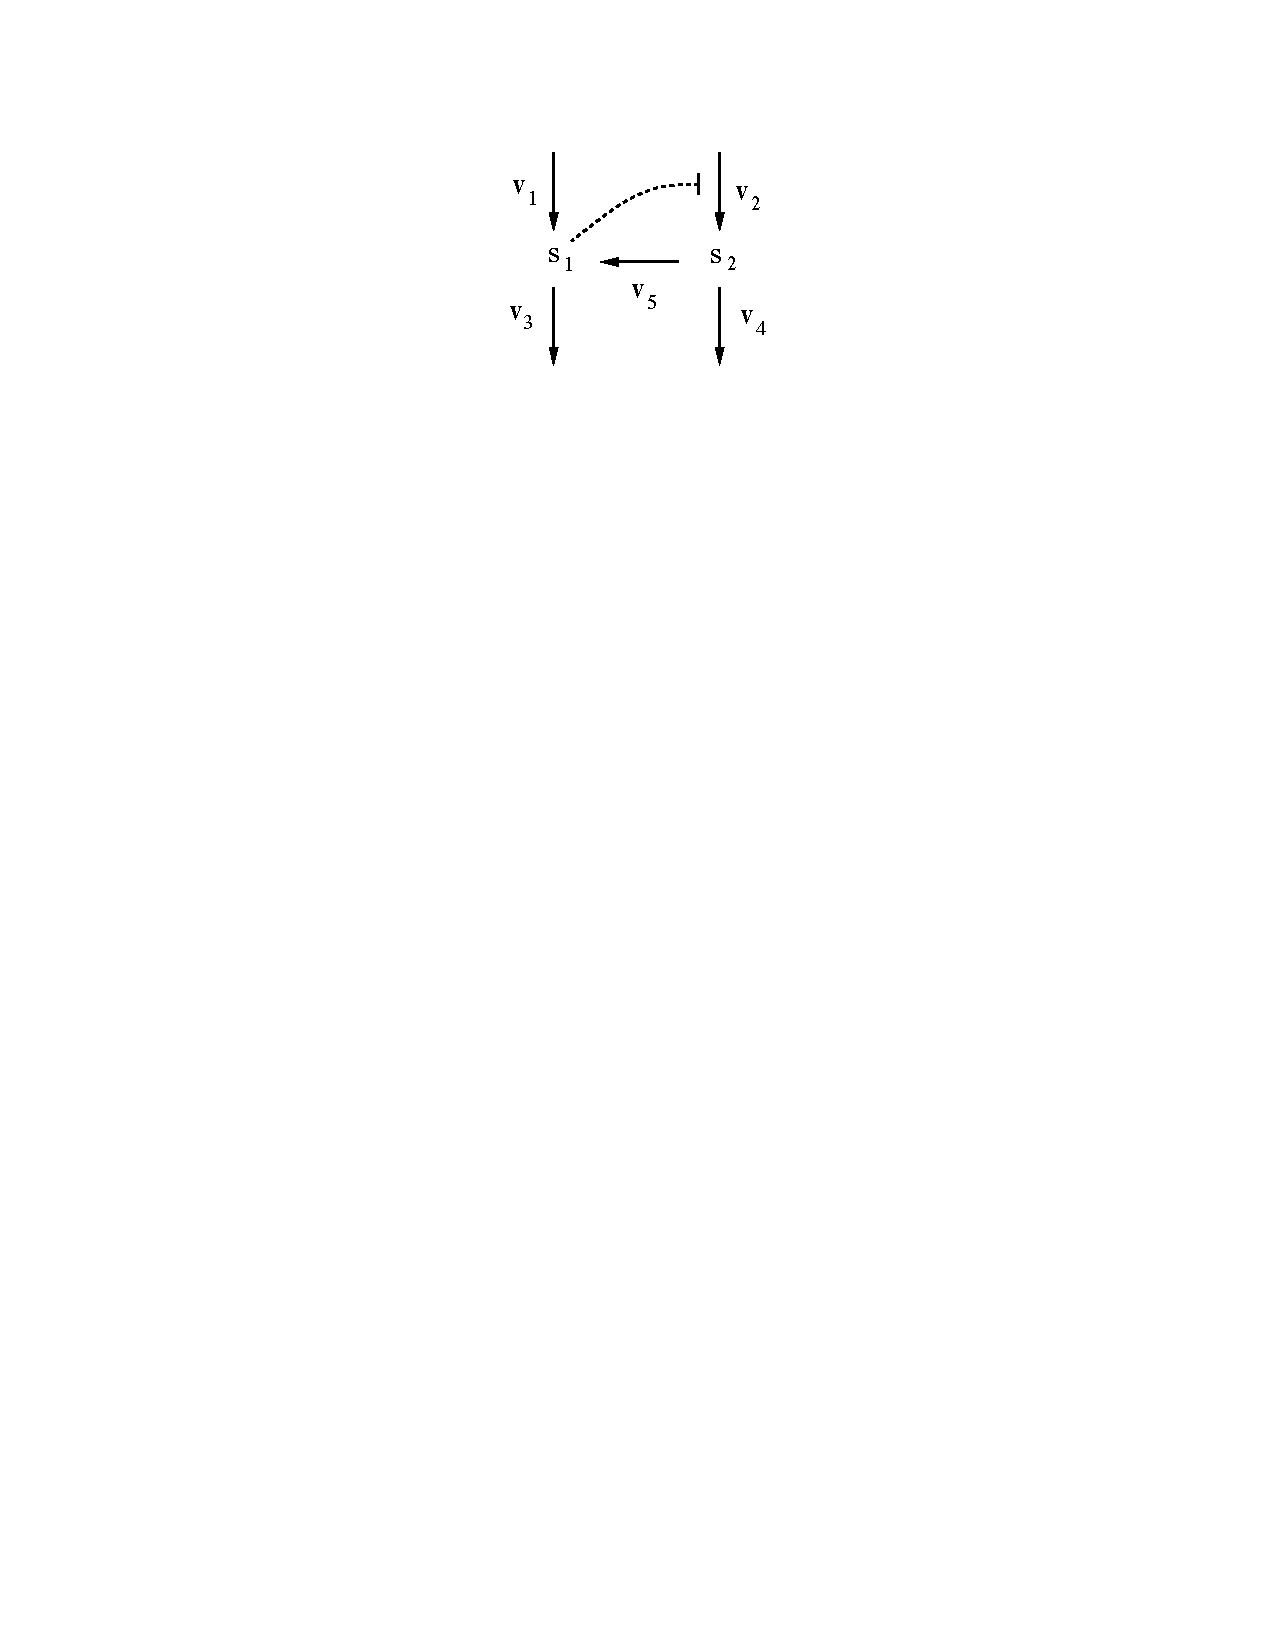
\includegraphics[width=2.5in]{networkhw4}
\end{center}
Take all reaction rates as mass action (with rate constants as specified), except for the inhibited reaction, which has rate 
$$\frac{k_2}{1+s_1^2}.$$
\begin{enumerate}
\item Find general equations for the $s_1$- and $s_2$-nullclines. \\
\item Fix the parameters as $k_1=1$ mM/min, $k_3=1$/min, $k_2=20$ mM/min, $k_4=1$/min, $k_5=2$/min.  Draw, by hand, a sketch of the system's phase portrait.  On your phase portrait, label the four regions of the phase space in which the trajectories increase/decrease in concentrations $s_1$ and $s_2$.  (This can be accomplished by determining the direction of motion along each nullcline, on each side of the equilibrium).
\end{enumerate}

\item Turn in the problem that we did in class:
\begin{center}
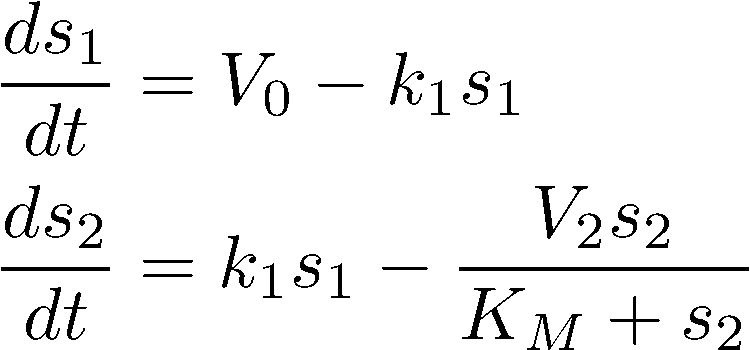
\includegraphics[width=1.5in]{classprob}
\end{center}
\begin{enumerate}
\item Identify the steady state
\item Construct the system Jacobian at the steady by taking partial derivatives and evaluating
\item Compute the eigenvalues of the Jacobian (Hint: if there are zeros off the diagonal, then the eigenvalues are just the diagonal elements! (Can also use matlab if you’re not sure)
 \item Check the sign of their real parts and determine stability
\end{enumerate}


\item {\bf Sensitivity analysis: reversible reaction.} Consider the reversible reaction
\beqn
A \autorightleftharpoons{$k_1$}{$k_2$} A^*
\eeqn
with mass-action rate constants as shown.
Let $T$ be the total concentration of $A$ and $A^*$.  
\newline
\begin{enumerate}
\item Solve for the steady-state concentration of $A^*$ and verify (just explain in words) that an increase in $k_1$ leads to an increase in $[A^*]^{ss}$.

\item Use parametric sensitivity analysis to determine whether the steady state concentration of $A^*$ is more sensitive to a 1\% increase in $T$ or a 1\% increase in $k_1$.  Does the answer depend on the values of the parameters?
\end{enumerate}


\end{enumerate}

\end{document} 

\newpage
